% !TEX root = ./presentation_screen.tex
% !TEX encoding = UTF-8
%
\usepackage{csquotes}
\usepackage[texencoding=utf8,backend=biber,style=authoryear-comp,bibstyle=authoryear,citestyle=authoryear-comp]{biblatex}


\usepackage[english]{babel} 
\usepackage{amssymb,amsmath,amsbsy,mathrsfs}
\usepackage{ulem}
\renewcommand<>{\sout}[1]{
  \only#2{\beameroriginal{\sout}{#1}}
  \invisible#2{#1}
}

\usepackage[SchoolofElectricalEngineering]{aaltologo}
\DeclareRobustCommand{\AaltoLogoRandomize}[1][rby]{%
\setcounter{aaltologo_color}{2}\gdef\AaltoLogoColor{aaltoBlue}%
\setcounter{aaltologo_mark}{1}\gdef\AaltoLogoMark{?}%
}

% Now set the theme
\usetheme[invariant,sidebar,school=SchoolofElectricalEngineering]{Aalto}
%\usetheme{Aalto}

%\usepackage[utf8]{inputenc}

\usepackage{tikz}

\usetikzlibrary{shapes.geometric,positioning,calc,fit,matrix,decorations.pathmorphing}
\usepackage{tikz-qtree}
\usepackage{graphicx}
\setbeamerfont{footnote}{size=\tiny}

\newcommand{\ns}{Northern Sámi}
\newcommand{\ngram}{$n$-gram}

\newcommand{\ds}[1]{\textsc{#1}}

\bibliography{../mybib}

\title{Automatic Speech Recognition for \ns\ with comparison to other Uralic Languages}
%\subtitle{Computational pragmatics}
%\subtitle[Chpt 11.5,13]{Techniques for Noise Robustness in Automatic Speech Recognition, Chapter 11.5 \& 13}
\author[Peter Smit]{Peter Smit, Juho Leinonen, Kristiina Jokinen, Mikko Kurimo}
\institute[Aalto University/Helsinki University]{Aalto University \\ Helsinki University}
\date{January 20, 2016}


\begin{document}
\begin{frame}
\titlepage
\end{frame}

%\section{Introduction}
%\begin{frame}
%\frametitle{Spoken Dialogue}
%
%\begin{itemize}
%\item For face recognition we would like faces to be on the same alignment
%\end{itemize}
%\end{frame}
\begin{frame}
\frametitle{Aalto University Speech Recognition Research Group}
\begin{itemize}
\item Former Helsinki University of Technology
\item Prof. Mikko Kurimo
\item Broad-ranged research in Speech Recognition and Language Modeling, with special focus on Finnish
\item Home of Morfessor\\[1cm]
\item Speech technology for under-resourced languages
\end{itemize}
\end{frame}


\begin{frame}
\frametitle{Contents}
\tableofcontents
\end{frame}

%\section{Morfessor Categories MAP}




\section{A diaglogue system for Northern Sami}
\begin{frame}
\frametitle{A diaglogue system for Northern Sami}
\begin{itemize}
\item WikiTalk for \ns
\item Kids ask questions from Robot, and the Robot gives information by reading Wikipedia articles to them
\item Speech recognition (ASR) and speech synthesis (TTS) are needed for this application
\end{itemize}
\end{frame}

\begin{frame}
\frametitle{Previous work}
\begin{itemize}
\item Commercial Speech Synthesis system by Acapela Group\\
\item Linguistic databases and tools by University of Tromsø\\[1cm]
\item Master's thesis by Leinonen (2015)\\
\end{itemize}
\end{frame}

\begin{frame}
\frametitle{Speech Technology for Northern Sami - Challenges}
\begin{itemize}
\item Only a limited amount of data is available for making ASR/TTS models
\end{itemize}
\end{frame}



\section[Speech Recognition]{Automatic Speech Recognition (ASR)}
\begin{frame}
\frametitle{What is needed for speech recognition?}
\begin{itemize}
\item Corpus of aligned audio and text
\item Big corpus of text data for language modeling
\item Dictionaries/lexicons (or the expertise to generate them)
\item Phonetic question sets (for decision tree clustering)
\end{itemize}
\end{frame}

\begin{frame}
\frametitle{Speaker-independent vs Speaker-dependent ASR}
\begin{itemize}
\item Speaker-independent (SI) systems works for any speaker of a language
\item Speaker-dependent (SD) systems  only works for the training speaker
\item SI systems need audio data from many different speakers (50-100 for decent results)
\item SD system only needs data from a single speaker
\end{itemize}
\end{frame}


\section[Under-resourced]{ASR for Under-Resourced languages}
\begin{frame}
\frametitle{Challenges for Under-resourced Languages}
\begin{itemize}
\item Audio Data
\item Text Data
\item Expertise
\end{itemize}
\end{frame}
%

\begin{frame}
\frametitle{Solutions for Under-resourced Languages}
\begin{itemize}
\item Audio Data
\begin{itemize}
\item Audio books
\end{itemize}
\item Text Data
\begin{itemize}
\item Web scraping
\end{itemize}
\item Expertise
\begin{itemize}
\item Unsupervised methods
\item Bootstrapping on related languages
\end{itemize}
\end{itemize}
\end{frame}

\section{Experiments}
\begin{frame}
\frametitle{\ns\ model with Wikipedia language model}

\begin{tabular}{ll|rrr|rrr}
& & \textbf{Speaker SF1} & \textbf{Speaker SM1} \\
 \textbf{Unit} & \textbf{Toolkit} & \textbf{9-gram} & \textbf{9-gram}\\\hline
 words & SRILM & 52.9 / 12.7&  48.7 / 11.1\\
morphs & SRILM & 39.1 / 9.1 &  37.3 / 8.5 \\
 morphs & VariKN   & 37.6 / 8.7 & 34.1 / 7.9 \\
%DST & words & SRILM & & & & & & \\
%DST & morphs & SRILM & & & & & & \\
%DST & morphs & VariKN  & & & & &  & \\ 

\end{tabular}
\\[1cm]
Word error rate / Letter error rate\\
\end{frame}

\begin{frame}
\frametitle{\ns\ model with Big language model}
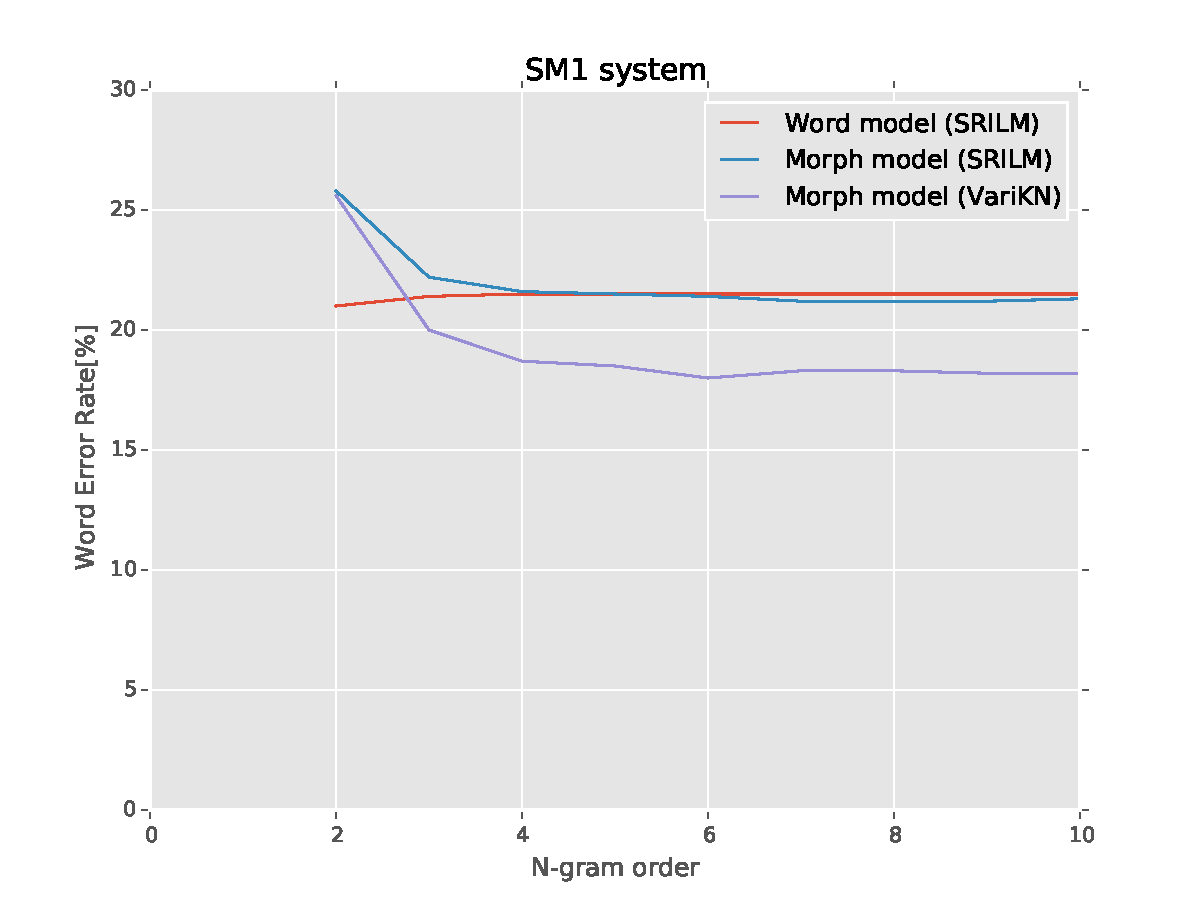
\includegraphics[width=.86\textwidth]{../figures/sme1}

\end{frame}

\begin{frame}
\frametitle{Comparison to other Uralic Languages}
\begin{tabular}{llp{4cm}r}
 \textbf{Language} & \textbf{Gender} & \textbf{Title} & \textbf{Hours}\\\hline
Estonian & Female &Nils Holgerssoni imeline teekond läbi Rootsi  & 16\\
 Estonian & Male & Würst Gabriel ehk Pirita kloostri wiimsed päewad & 6\\
 Finnish & Female & Syntymättömien sukupolvien Eurooppa & 12\\
 Finnish & Male & Seitsemän veljestä & 13\\
N-Sámi & Female & UIT-SME-TTSF & 3.3\\
 N-Sámi & Male & UIT-SME-TTSM & 4.6\\
\end{tabular}
\end{frame}

\begin{frame}
\frametitle{Comparison to other Uralic Languages}
2.5 hours of audio data 
\begin{tabular}{ll|rr|rr}
 & & \multicolumn{2}{|c|}{\textbf{\ds{Train+Wiki}}}  & \multicolumn{2}{|c}{\textbf{\ds{Big}}}\\
\textbf{Language} & \textbf{Voice} & \textbf{WER} & \textbf{LER}& \textbf{{WER}} & \textbf{LER}\\\hline
Estonian & EF1 & 39.6 & 15.8 & 25.0 & 11.4\\
Estonian & EM1 & 39.2 & 13.3 & 25.5 & 9.6\\
Finnish & FF1 & 25.2 &4.1& 8.9 & 2.1  \\
Finnish & FM1 & 35.8 & 7.7 & 24.9 &  5.6 \\
\ns & SF1 & 37.5 & 8.5 & 23.7  & 5.5 \\
\ns & SM1 & 39.5 & 9.4& 20.9 & 4.9  \\
\end{tabular}
\end{frame}



\begin{frame}
\frametitle{Comparison to other Uralic Languages}
\begin{tabular}{lr|rr|rr}
 & & \multicolumn{2}{|c}{\textbf{2.5 hours}} & \multicolumn{2}{|c}{\textbf{All data}} \\
 \textbf{Voice} & \textbf{\#hours}  & \textbf{WER} & \textbf{LER}& \textbf{{WER}} & \textbf{LER} \\\hline %& \textbf{\%+ hours} & \textbf{-WER/hour} \\\hline
 EF1 & 8 & 25.0  & 11.4 & 18.8 & 8.3  \\
 EM1& 4.5&25.5 & 9.6  & 23.2 & 8.4  \\
 FF1 & 9  & 8.9 & 2.1  & 8.1 &  1.9  \\
 FM1 & 10 & 24.9 & 5.6  & 19.8  & 3.7    \\
SF1 & 2.5    & 23.7  & 5.5  & 23.7  & 5.5  \\
SM1 & 3.5 & 20.9 & 4.9  & 18.1  & 4.2   \\
\end{tabular}
\end{frame}


\begin{frame}
\frametitle{State-of-the art Uralic Languages}
\begin{tabular}{llrrl}
\textbf{Language} & \textbf{Description} & \textbf{WER} & \textbf{LER} & \textbf{}\\\hline
Estonian & Broadcast conversations  & 17.9\% & &  \footfullcite{alumae2014recent} \\
Estonian & Oral presentations  & 26.3\% & &  \\
Finnish & Speecon testset  & & 2.9\%&  \footfullcite{pylkkonen2012} \\
Estonian & Telephone speech &33.1\% & 11.9\% & \footfullcite{hirsimaki2009importance}\\
Finnish & Telephone speech & 21.6\% & 6.8\% & \\
\end{tabular}
\end{frame}

\begin{frame}
\frametitle{Future work}
\begin{itemize}
\item Expand recognizer to be Speaker Independent
\end{itemize}

\end{frame}
\section*{Video}
\begin{frame}
\frametitle{Video}
\begin{center}
\url{https://youtu.be/14jYeViJ0X0}
\end{center}
\end{frame}


\section*{Questions}

\begin{frame}
\frametitle{Questions}
\begin{center}
Questions?
\end{center}
\end{frame}


%\begin{frame}[allowframebreaks]
%\printbibliography
%
%\end{frame}
%


\end{document}